%\documentclass[../main.tex]{subfiles}

\section{Introduction}
\label{sec:intro}

Applications across a broad swath of domains use linear algebra to represent geometry, coordinates, and simulations of the physical world.
Scientific computing workloads, robotics control software, and real-time graphics renderers all use matrices and vectors pervasively to manipulate points according to linear-algebraic laws.
The programming languages that express these computations, however, rarely capture the underlying \emph{geometric} properties of these operations.
In domains where performance is critical, most languages provide only thin abstractions over the low-level vector and matrix data types that the underlying hardware (i.e., GPU) implements.
A typical language might have a basic \code{vec2} data type for vectors consisting of two floating-point numbers, for example, but not distinguish between 2D vectors in rectangular or polar coordinates---or between points in differently scaled rectangular coordinate systems.

This paper focuses on real-time 3D rendering on GPUs, where correctness hazards in linear algebra code are particularly pervasive.
The central problem is that graphics code frequently entangles application logic with abstract geometric reasoning. Programs must juggle vectors from a multitude of distinct coordinate systems while simultaneously optimizing for performance.
This conflation of abstraction and implementation concerns makes it easy to confuse different coordinate system representations and to introduce subtle bugs.
Figure~\ref{fig:bunnyimages} shows an example: a coordinate system handling bug yields incorrect visual output that would be difficult to catch with testing.

\subsection{The Problem}

\begin{figure}
\begin{minipage}{.48\linewidth}
\centering
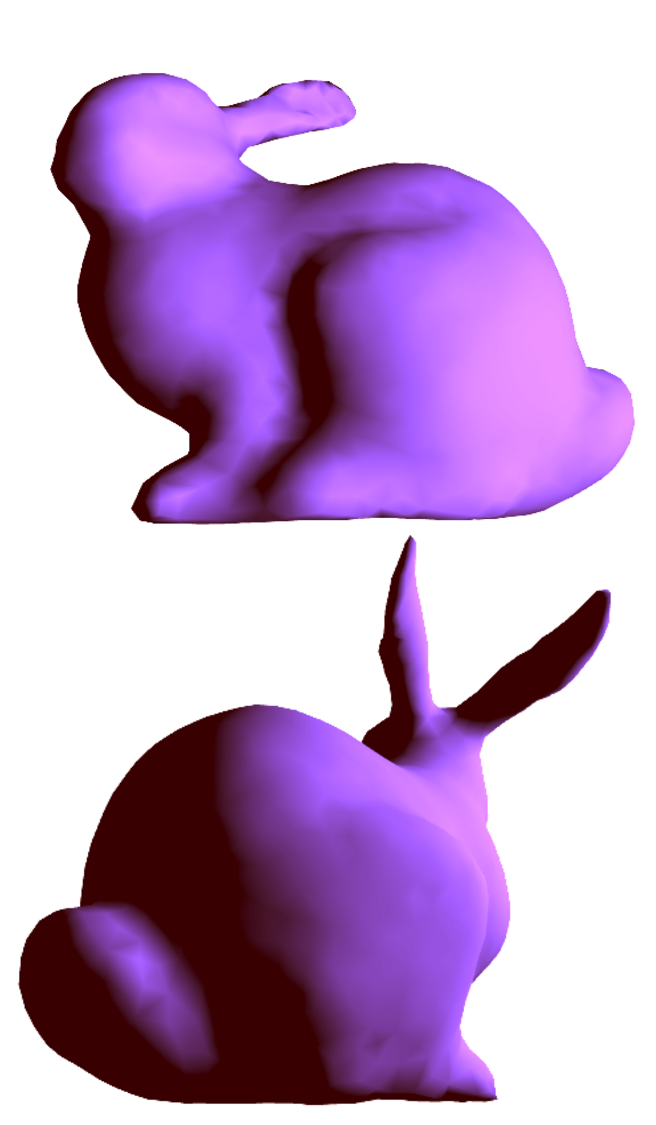
\includegraphics[scale=0.25]{fig/goodbunnies.pdf}
\caption{Correct implementation.}
\label{fig:bunnygood}
\end{minipage}
\begin{minipage}{.48\linewidth}
	\centering
	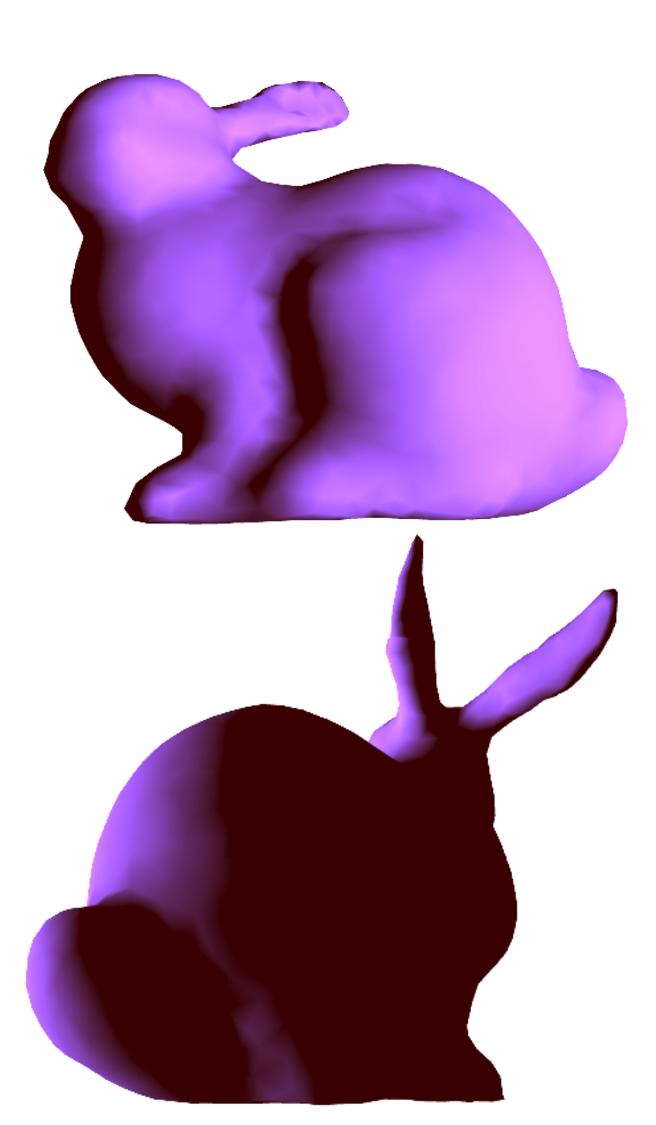
\includegraphics[scale=0.25]{fig/badbunnies.pdf}
	\caption{Incorrect implementation.}
	\label{fig:bunnybad}
\end{minipage}
\caption{Objects rendered with an implementation of the diffuse component of Phong lighting~\cite{phong},
% where the light source is fixed to the top right of the screen,
without (a) and with (b) a coordinate system transformation bug.
The root cause is an incorrect spatial translation of the light source.
The problem is only visible from one side of the model.}
\end{figure}
\begin{figure}
\centering
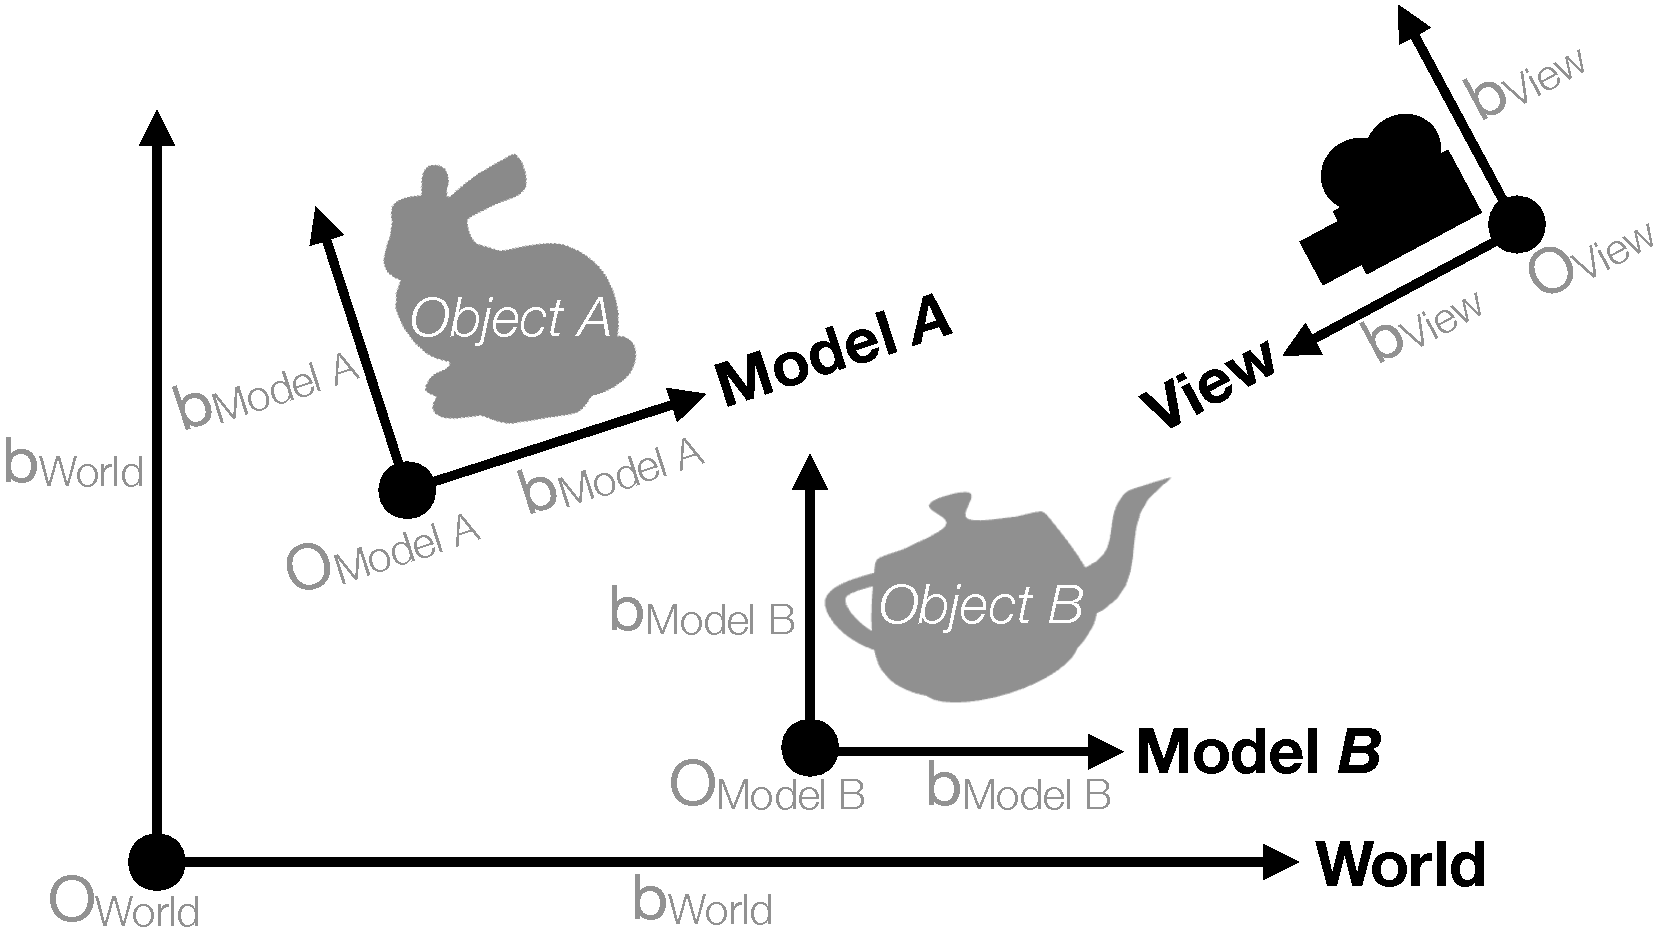
\includegraphics[width=\linewidth]{fig/coordinate-spaces-2.pdf}
\caption{Coordinate systems in graphics code.
	\textbf{Model A}, \textbf{Model B}, \textbf{World}, and \textbf{View} are coordinate systems.
	A coordinate system is defined by its basis vectors $b$ and origin $O$.
	% Ridiculous LaTeX note: the underscores in $b_s$ and $O_s$ were causing labeling issues. I reworded this to just refer to $b$ and $O$ by themselves to avoid this. I think it reads clearly enough this way. --A
	The \textbf{View} represents the perspective of a simulated camera.
	% Deleted the below because it doesn't seem 100% relevant.
	% Applications perform geometric operations on objects in either world or view space, depending on whether these operations require information about the viewer.
}
\label{fig:spaces}
\end{figure}

Coordinate systems proliferate in graphics programming because 3D scenes consist of many individual objects.
Figure~\ref{fig:spaces} depicts a standard setup for rendering two objects in a single scene.
Each object comes specified as a \emph{mesh}, which consists of coordinate vectors for each vertex position.
The mesh provides these vectors in a local, object-specific coordinate system called \emph{model} space.
The application positions multiple objects relative to one another in \emph{world} space,
and the simulated camera's position and angle define a \emph{view} space.

Renderer code needs to combine vectors from different coordinate systems, such as in this distance calculation:
%
\begin{lstlisting}
float dist = length(teapotVertex - bunnyVertex);
\end{lstlisting}
%
This code may be incorrect, however, depending on the representation of the \code{teapotVertex} and \code{bunnyVertex} vectors.
If the values come from the mesh data, they are each represented in their respective model spaces---and subtracting them yields a geometrically meaningless result.
A correct computation needs to convert the operands into a common coordinate system using \emph{affine transformation} matrices:
%
\begin{lstlisting}
float dist = length(teapotToWorld * teapotVertex - 
	bunnyToWorld * bunnyVertex);
\end{lstlisting}
%
Here, the \code{teapotToWorld} and \code{bunnyToWorld} matrices define the transformations from each model space into world space.

\paragraph{Geometry bugs are hard to catch.}

Mainstream rendering languages like OpenGL's GLSL~\cite{opengl} cannot statically rule out coordinate system mismatches.
In GLSL, the variables \code{teapotVertex} and \code{bunnyVertex} would both have the type \code{vec3}, i.e., a tuple of three floating-point numbers.
%
These bugs are also hard to detect dynamically.
They do not crash programs---they only manifest in visual blemishes.
While the buggy output in Figure~\ref{fig:bunnybad} clearly differs from the correct output in Figure~\ref{fig:bunnygood}, it can be unclear what has gone wrong---or, when examining the buggy output alone, that anything has gone wrong at all.
Accordingly, writing assertions or unit tests to catch this kind of bug can be challenging: specifying the behavior of a graphics program requires formalizing how the resulting scene should be perceived.
Viewers can perceive many possible outputs as visually indistinguishable, so even an informal specification of what makes a renderer ``correct,'' for documentation or testing, can be difficult to write.

\paragraph{Geometry bugs in the wild.}

Even among established graphics libraries, geometry bugs can remain latent until a seemingly correct API change reveals the bug.
% For example, in LÖVR, a framework for rapidly building VR experiences, the developers discovered a bug where a variable that was in one space was being used as if it was in another.\footnote{\url{https://github.com/bjornbytes/lovr/issues/55}}
This bug lay dormant while, to quote one of the maintainers, ``there was a change in the rendering method that amplified the problems caused by this.'' The maintainer then noted that they needed to ``go backfill this fix to all the docs/examples that have the broken version.''
Because their effects are hard to detect, geometry bugs can persist and cause subtle inaccuracies that grow as code evolves.

We found similar issues that arise when APIs fail to specify information about vector spaces.
% In the Processing graphical IDE, for example, confusion surrounding a camera API led to a 20-comment thread before a developer concluded that ``better documentation could alleviate this to some extent: it needs to be clear that modelspace is relative to the camera at the time of construction.''\footnote{\url{https://github.com/processing/processing/issues/187}}
% And in the visualization library GLVisualize.jl, users disagree about the space that the library uses for a light position.\footnote{\url{https://github.com/JuliaGL/GLVisualize.jl/pull/188}}
The root cause in both cases is that the programming language affords no opportunity to convey vector space information.

This paper advocates for making geometric spaces manifest in programs themselves via a type system.
Language support for geometric spaces can remove ambiguity and provide self-documenting interfaces between parts of a program.
Static type checking can automatically enforce preconditions on geometric operations that would otherwise be left unchecked.


\subsection{Geometry Types}

We introduce a type system that can eliminate this class of bugs, and we describe a mechanism for automatic transformation that can rule out some of them by construction.
\emph{Geometry types} describe the coordinate system representing each value and the transformations that manipulate them.
A geometry type encodes three components:
the \emph{reference frame}, such as model, world, or view space;
the \emph{geometric object}, such as a point or a direction;
and the \emph{coordinate scheme}, such as Cartesian or spherical coordinates.
Together, these components define which geometric operations are legal and how to implement them.

The core contribution of this paper is that all three components of geometry types are necessary.  
The three aspects interact in subtle ways, and real-world graphics rendering code varies in each component.
Simpler systems that only use a single label~\cite{safegi} cannot express the full flexibility of realistic rendering code and cannot cleanly support automatic transformations.
We show how encoding geometry types in a real system can help avoid and eliminate realistic geometry bugs.
We will explore further how these components are defined and interact to provide operation information in Section~\ref{sec:langlang}.

We design a language, Gator, that builds on geometry types to rule out coordinate system bugs and to automatically generate correct transformation code.
In Gator, programmers can write \code{teapotVertex in world} to obtain a representation of the \code{teapotVertex} vector in the \code{world} reference frame.
% The Gator compiler finds the appropriate sequence of matrix--vector multiplications necessary to produce a result of the correct type.
The end result is a higher-level programming model that lets programmers focus on the geometric semantics of their programs without sacrificing efficiency.

We implement Gator as an overlay on GLSL~\cite{glsl}, a popular language for implementing shaders in real-time graphics pipelines.
Most GLSL programs are also valid in Gator, so programmers can easily port existing code and incrementally add typing annotations to improve its safety.
We formalize a geometry type system and show that erasing these types preserves soundness.
In our evaluation, we port rendering programs from GLSL to qualitatively explore Gator's expressiveness and its ability to rule out geometry bugs.
We also quantitatively compare the applications to standard GLSL implementations and find that Gator's automatic generation of transformation code does not yield meaningfully slower rendering time than hand-tuned (and unsafe) GLSL code.

This paper's contributions are:
%
\begin{itemize}
\item We identify a class of geometry bugs that exist in geometry-heavy, linear-algebra-centric code such as physical simulations and graphics renderers.
\item We design a type system to describe latent coordinate systems present in linear algebra computations and prevents geometry bugs.
\item We introduce a language construct that builds on the type system to automatically generate transformation code that is type correct by construction.
\item We implement the type system and automatic transformation feature in Gator, an overlay on the GLSL language that powers all OpenGL-based 3D rendering.
\item We experiment with case studies in the form of real graphics rendering code to show how Gator can express common patterns and prevent bugs with minimal performance overhead.
\end{itemize}
%
We begin with some background via a running example
before describing Gator in detail.


\section{Running Example: Diffuse Shading}
\label{sec:example}

This section introduces the concept of geometry bugs via an example:
we implement \emph{diffuse lighting}, a component of the classic Phong lighting model~\cite{phong}.\footnote{Appendix A gives a complete GLSL implementation of the Phong model.}
We assume some basic linear algebra concepts but no background in graphics or rendering.

\subsection{Gentle Introduction to Shader Programming}
Shader programs are code, typically written in C-like languages such as GLSL or HLSL, that runs on the GPU to render a graphics \emph{scene}. The GPU executes a pipeline of shader programs, where each shader is specialized to transform a certain property of a graphical object.  The shader pipeline consists of several stages.  The most notable of these stages are the vertex shader, which outputs the position of each vertex as a pixel and the fragment shader, which outputs the color of each \emph{fragment} corresponding to an on-screen pixel.

In graphics, the \emph{scene} is a collection of objects. The shape of an object is determined by mesh data consisting of \emph{position vectors} for each vertex, denoting the spatial structure of the object, and \emph{normal vectors}, denoting the surface orientation at each vertex. 

The kind of transformation each graphics shader applies to a graphical object depends on the pipeline stage. 
We focus on the vertex and fragment shader, the most common user-programmable stages of the graphics pipeline. 

\subsection{Diffuse Lighting} 

Diffuse lighting is a basic lighting model that simulates the local illumination on the surface of an object.
Given a point on an object, the intensity of its diffuse component is proportional to the angle between the position of the light ray and the local surface normal. 
The diffuse model first computes the direction of the light by subtracting the mesh (surface) position, \textit{fragPos}, from the light position:
%
\begin{align*}
\mathit{lightDir} &= \mathsf{normalize}(\mathit{lightPos} - \mathit{fragPos})
\end{align*}
%
We normalize the vector, which preserves the angle but sets the magnitude to 1. 
We calculate the resulting diffuse intensity at this fragment as the angle between the incoming light ray and the fragment normal using the vector dot product (which is algebraically the sum of the product of vector components):
%
\begin{align*}
\mathit{diffuse} &= \mathsf{max}(\mathit{lightDir}\cdot\mathit{fragNorm}, 0.)
\end{align*}
%
The \textsf{max} function used here prevents light from passing through the object by rejecting reflection angles greater than perpendicular.

\subsection{Where Things Go Wrong: GLSL Implementation}
\label{subsec:wrong}
To implement the diffuse lighting model, we must write a GLSL shader program that operates on a per-fragment basis. 
This section shows how this seemingly simple program translates to surprisingly complex code.
We identify pitfalls in this implementation process that our type system will address.

GLSL has vector and matrix types, with names like \code{vec3} and \code{mat4}, along with built-in vector functions that make an initial implementation of the diffuse component seem straightforward:
%
\begin{lstlisting}
float naiveDiffuse(vec3 lightPos, vec3 fragPos, vec3 fragNorm) {
  vec3 lightDir = normalize(lightPos - fragPos);
  return max(dot(lightDir, normalize(fragNorm)), 0.);
}
\end{lstlisting}
%
% Unfortunately, this na\"ive implementation has a bug because it fails to account for coordinate systems.
Although \code{lightPos} and \code{fragPos} have the same type, they are not geometrically compatible: real renderers need to represent them with different reference frames and coordinate schemes.
While this incorrect code directly reflects the mathematical description above, the output is nonetheless incorrect:
it produces the buggy output in Figure~\ref{fig:bunnybad}.

% \xxx[a]{Let's put a real quick transition paragraph here to say something like: ``Unfortunately, this naive implementation has lots of bugs that reveal disconnects between the mathematical description above and the more specific computational implementation. We will describe each of those problems, which will motivate Gator's language design...''}
% \xxx[dg]{Nah, there's really only one bug that leads to several issues.  I really like the transition straight into the issue here; that we're leading into what Gator does feels implicitly true by the structure of the section}

\paragraph{Coordinate Systems}
The underlying problem is that software needs to represent different vectors in different coordinate systems.
Information needed to render the shape of a single graphical object, the positions and normal vectors, lies in the object's \emph{model space}, as can be seen in Figure~\ref{fig:spaces}.
A model space represents the coordinates local to a single object in the scene.
The origin of this space is centered in the model, with basis vectors matching the model orientation and scale.
Both may change dynamically as time passes in the scene; however, each is fixed during a single iteration of the shader.
\emph{World space} gives the absolute coordinates for the entire scene, so the basis vectors and origin of world space are typically fixed.

Mesh data is scene independent, so we represent mesh parameters such as \code{fragPos} and \code{fragNorm} initially in model space, independent of the object's current relative position within the scene.
In contrast, we represent the position of a light source relative to the entire scene---so \code{lightPos} is in world space.
As a result, the subtraction expression \code{lightPos - fragPos} attempts to compare vectors represented in different spaces, yielding a geometrically meaningless result.
This bug produces the incorrect output seen in Figure~\ref{fig:bunnybad}.

\paragraph {Transformation Matrices} To fix this program, the shader needs to \emph{transform} the two vectors to a common coordinate system before subtracting them. 
Mathematically, coordinate systems define an affine space, and thus geometric transformations on coordinate systems can be linear or affine.
Affine transformations can change the origin and basis vectors, which can represent translation, while linear transformations affect only the basis vectors, which can represent rotation and scale. 

These geometric transformations are represented in code as \emph{transformation matrices}.
To apply a transformation to a vector, shader code uses matrix-vector multiplication. 
For example, the shader application may provide a matrix \code{uModel} that defines the transformation from model to world space using matrix multiplication:
\begin{lstlisting}
vec3 lightDir = normalize(lightPos - <@\textcolor{darkolivegreen}{uModel * }@>fragPos));
\end{lstlisting}

\paragraph{Homogeneous Coordinates}
Unfortunately, this matrix multiplication implementation introduces another bug.
Transforming \code{fragPos} from model to world space requires both a linear scaling and rotation transformation and a translation to account for change of origins.
This linear transformations with translation is represented by an \emph{affine transformation matrix}. 
This is a problem: an affine transformation matrix for 3D vectors must be represented as a $4\times4$ matrix. To multiply this matrix by \code{fragPos} (which is a 3-dimensional vector), we need a sensible representation of \code{fragPos} as a 4-dimensional vector.
It is thus not immediately clear by what vector we need to multiply:
%
\begin{lstlisting}
vec3 lightDir = normalize(lightPos - <@\textcolor{darkolivegreen}{vec3(uModel *}@><@\textcolor{red}{?}@><@\textcolor{darkolivegreen}{)}@>);
\end{lstlisting}
%
Because a 3$\times$3 Cartesian transformation matrix on 3-dimensional vectors can only express linear transformations, graphics software typically uses a second kind of coordinate system called \emph{homogeneous coordinates}.
An $n$-dimensional vector in homogeneous coordinates uses $n+1$ values: the underlying Cartesian coordinates and a \emph{scaling factor}, $w$.
A 4$\times$4 transformation matrix in homogeneous coordinates can express \emph{affine} transformations on the underlying 3-dimensional space, including translation.

To convert from Cartesian to homogeneous coordinates, a vector $[x, y, z]$ becomes $[x, y, z, 1.]$;
in the opposite direction, the homogeneous vector $[x, y, z, w]$ becomes $[x/w, y/w, z/w]$.
To fix our example to use the 4-dimensional affine transformation \code{uModel}, we can extend \code{fragPos} into a homogeneous \code{vec4} value:
%
\begin{lstlisting}
vec3 lightDir = normalize(
  lightPos - <@\textcolor{darkolivegreen}{vec3(uModel * vec4(}@>fragPos<@\textcolor{darkolivegreen}{, 1.))}@>
);
\end{lstlisting}
%
The GLSL functions \code{vec4} and \code{vec3} extend a 3-dimensional vector with the given component and truncate a 4-dimensional vector, respectively. We now have a \code{lightDir} in a consistent coordinate system, namely in the world space.

The final calculation of the diffuse intensity uses this expression:
%
\begin{lstlisting}
max(dot(lightDir, normalize(fragNorm)), 0.)
\end{lstlisting}
%
Here, \code{fragNorm} resides in model space and should be transformed into world space. One tricky detail, however, is that \code{fragNorm} denotes a \emph{direction}, as opposed to a \emph{position} as in \code{fragPos}. 
These require different geometric representations, because a direction should not be affected by translation. 
Fortunately, there is a trick to avoid this issue while still permitting the use of our nice homogeneous coordinate representation.
By extending \code{fragNorm} with $w = 0$, affine translation is not applied. 
%
\begin{lstlisting}
return max(dot(lightDir, normalize(
  <@\textcolor{darkolivegreen}{vec3(uModel * vec4(}@>fragNorm<@\textcolor{darkolivegreen}{, 0.))}@>
);
\end{lstlisting}
%
This subtle difference is a common source of errors, particularly for novice programmers. 
Finally, we have a correct GLSL implementation of \code{diffuse}. This version results in the correct output in Figure~\ref{fig:bunnygood}. 

\section{Geometry Types}
\label{sec:langlang}

The problems in the previous section arise from the gap between the abstract math and the concrete implementation in code.
We classify this kind of bug, when code performs geometrically meaningless operations, as a \emph{geometry error}.
Gator provides a framework for declaring a type system that can define and catch geometry errors in programs.

The core concept in Gator is the introduction of \emph{geometry types}.
These types refine simple GLSL-like vector data types, such as \code{vec3} and \code{mat4}, with information about the geometric object they represent.
A geometry type consists of three components:
%
\begin{itemize}
\item The \emph{reference frame} defines the position and orientation of the coordinate system. A reference frame is determined by its basis vectors and origin. Examples of reference frames are model, world, and projective space. 
\item The \emph{coordinate scheme} describes a coordinate system by providing operation and object definitions, such as homogeneous and Cartesian coordinates. Coordinate schemes expresses how to represent an abstract value computationally, which identifies what the underlying GLSL-like type is.
\item The \emph{geometric object} describes which geometric construct the data represents, such as a point, vector, or transformation.
\end{itemize}
%
In Gator, the syntax for a geometry type is 
%
\code{scheme<frame>.object}
%
This notation invokes both module members and parametric polymorphism.
Coordinate schemes are parameterized by a reference frame, while geometric objects are member types of a parameterized scheme.
For example, \code{cart3<world>.point} is the type of a point lying in world space represented in a 3D Cartesian coordinate scheme.

The three geometry type components suffice to rule out the errors described in Section~\ref{sec:example}.
The rest of the section details each component. 

\subsection{Reference Frames}
\label{subsec:geotypes}
We can enhance the mathematical diffuse light computation above using geometry types:
%
\begin{lstlisting}
float diffuseNaive(
  <@\textcolor{darkolivegreen}{cart3<world>.point}@> lightPos, 
  <@\textcolor{darkolivegreen}{cart3<model>.point}@> fragPos, 
  <@\textcolor{darkolivegreen}{cart3<model>.direction}@> fragNorm) {
    cart3<world>.direction lightDir = 
      normalize(lightPos - fragPos);
    return max(dot(lightDir, normalize(fragNorm)), 0.0);
}
\end{lstlisting}
%
With these stronger types, the expression \code{lightPos - fragPos} in this function is an error, since \code{lightPos} and \code{fragPos} are in different frames. 
It is geometrically legal to subtract two positions to produce a vector; the only issue with this code is the difference of reference frames.  
We will further discuss how Gator determines subtraction is legal in Section~\ref{subsec:schemes}.

\paragraph{Definition}
Reference frames in Gator are labels with an integer dimension.  The dimension of a frame specifies the number of linearly independent basis vectors which make up the frame. Gator does not require explicit basis vectors for constructing frames; keeping basis vectors implicit helps minimize programmer requirements and helps avoid cluttering definitions with information we don't really need.
We will discuss what keeps these basis vectors are implicit through transformations between reference frames in Section~\ref{sec:in}.

The Gator syntax to declare the three-dimensional model and world frames is:
%
\begin{lstlisting}
frame model has dimension 3;
frame world has dimension 3;
\end{lstlisting}
%
\subsection{Coordinate Schemes}
\label{subsec:schemes}

To transform \code{fragPos} and \code{fragNormal} to the \code{world} reference frame, we need to provide an affine transformation matrix \code{uModel}.
%
\begin{lstlisting}
float diffuse(
  cart3<world>.point lightPos, 
  cart3<model>.point fragPos, 
  cart3<model>.direction fragNorm,
    <@\textcolor{darkolivegreen}{hom3<model>}@>.transformation<world> uModel) {
  cart3<world>.direction lightDir = 
    normalize(lightPos - (uModel * fragPos));
  return max(dot(lightDir, 
    normalize(<@\textcolor{darkolivegreen}{uModel *} fragNorm)), 0.0);
}
\end{lstlisting}
%
For this example, we define matrix--vector multiplication \code{$m$ * $v$} to update types akin to function application: it ensures that $m$ is a transformation in the same frame as the vector and parameterized on the destination frame $f$, then produces an output direction in the frame $f$.
With this definition, multiplying \code{uModel} by an object in the \code{model} reference frame will result in an object in the \code{world} frame.

Unfortunately, multiplying \code{uModel * fragPos} produces a Gator type error since \code{uModel} and \code{fragPos} are in different coordinate schemes.
We will resolve this issue in the next subsection by converting between schemes.

\paragraph{Definition}
Coordinate schemes provide definitions of geometric objects and operations.
Concretely, they consist of operation type declarations and concrete definitions for member objects and operations.
Geometric operations defined in coordinate schemes are expected to provide geometrically correct code, and are generally intended (though not required) to operate between objects within the coordinate scheme.
Recall that, instead of ``baking in'' a particular notion of geometry, Gator lets coordinate schemes provide types that define correctness for a given set of geometric operations.
%
\begin{lstlisting}
with frame(3) r:
coordinate cart3 : geometry {
  object vector is float[3];
  ...
}
\end{lstlisting}
For example, we can define 3D vector addition in Cartesian coordinates, which consists of adding the components of two vectors together.
\begin{lstlisting}
vector +(vector v1, vector v2) {
   return [v1[0] + v2[0], v1[1] + v2[1], v1[2] + v2[2]];
}
\end{lstlisting}
%
All coordinate schemes are required to be parameterized with reference frames, so \code{cart3<model>} and \code{cart3<world>} are different instantiations of the same scheme.
Gator's \code{with} syntax provides parametric polymorphism in the usual sense; in this example, the 3-dimensional Cartesian coordinate scheme is polymorphic over all 3-dimensional reference frames.

\subsection{Geometric Objects}
\label{subsec:objects}

To apply the \code{uModel} affine transformation to our position and normal, we first need to convert each to homogeneous coordinates.  Recall from Section~\ref{subsec:wrong}, however, that this coordinate system transformation \emph{differs for points and directions}.
To capture this distinction, we introduce the overloaded function \code{homify}:\footnote{For simplicity, this example \code{homify} is written only for objects in the \code{model} frame.  Gator supports function parameterization on reference frames, so we would normally write \code{homify} to work on any frame.}
%
\begin{lstlisting}
hom<model>.point homify(cart3<model>.point p) {
  return [p[0], p[1], p[2], 1.]; 
} 
hom<model>.direction homify(cart3<model>.direction p) {
  return [p[0], p[1], p[2], 0.]; 
}
\end{lstlisting}
%
Unlike Cartesian coordinates, homogeneous coordinates have different representations for points and directions: the latter must have zero for its last coordinate, $w$.

To send \code{fragPos} and \code{fragNorm} to homogeneous coordinates, it suffices to call \code{homify} and let the Gator compiler select the correct overloaded variant:
%
\begin{lstlisting}
homify(fragPos);  // Extends fragPos with w=1.
homify(fragNorm); // Extends fragNorm with w=0.
\end{lstlisting}  
%
We repeat this process to define the function \code{reduce}, which maps homogeneous to Cartesian coordinates.  Finally, we apply these functions to our model:
%
\begin{lstlisting}
float diffuse(
  cart3<world>.point lightPos, 
  cart3<model>.point fragPos, 
  cart3<model>.direction fragNorm,
    hom3<model>}.transformation<world> uModel) {
    cart3<world>.direction lightDir = normalize(lightPos - 
      <@\textcolor{darkolivegreen}{reduce}@>(uModel * <@\textcolor{darkolivegreen}{homify(}@>fragPos<@\textcolor{darkolivegreen}{)}@>));
  return max(dot(lightDir,
    normalize(<@\textcolor{darkolivegreen}{reduce}@>(uModel * <@\textcolor{darkolivegreen}{homify(}@>fragNorm)))
    0.0));
}
\end{lstlisting}
%
Now, by using all three components of the geometry type, our code will compile and produce the correct Phong diffuse color shown in Figure~\ref{fig:bunnygood}.

\paragraph{Definition}
The object component of a geometry type describes the type's underlying datatype and provides information on permitted operations.  
Object type definitions can be parameterized on reference frames, such as writing affine transformations \textit{to} a specific frame.
For example, we can define some objects in homogeneous coordinates:
%
\begin{lstlisting}
coordinate hom3 : geometry {
  object point is float[4];
  object direction is float[4];
  with frame(3) r:
  object transformation is float[4][4];
  ...
}
\end{lstlisting}
%
Object and type declarations in Gator extend existing types; for example, here \code{point} is defined as a subtype of \code{float[4]}.
When an operation is applied to one or more objects, Gator requires that they have matching coordinate schemes and that the function being applied has a definition in this matching scheme.
For example, by omitting a definition for addition between \code{point}s and their supertypes, we ensure that Gator will reject \code{fragPos +} \code{fragPos}.

\section{Automatic Transformations}
\label{sec:in}

Gator's type system statically rules out bad coordinate system transformation code.
In this section, we show how it can also help automatically generate transformation code that is correct by construction.
The idea is to raise the level of abstraction for coordinate system transformations so programmers do not write concrete matrix--vector multiplication computations---instead, they declaratively express source and destination spaces and let the compiler find the right transformations.
% Transformations between coordinate schemes and reference frames may require several steps, each of which is uniquely defined by the initial and target frames.
% As a result, writing down the functions to change an object's geometry type is often a purely mechanical task.
A declarative approach can obviate complex transformation code that
obscures the underlying computation and can quickly become out of date, such as this shift from \code{model} to \code{world} space:
% Transforming between \code{model} and \code{world} is a simple example of these challenges, requiring two function calls and a matrix multiplication each time we apply this transformation:
%
\begin{lstlisting}
cartesian<world>.direction worldNorm = 
  normalize(lightPos - reduce(uModel * homify(fragNorm)));
\end{lstlisting}
%
%\xxx[dg]{Give more intuition for why in expressions are useful and a viable abstraction in this context}
We extend Gator with an \code{in} expression that generates equivalent code automatically:
%
\begin{lstlisting}
cartesian<world>.direction worldNorm = 
  normalize(lightPos - fragNorm in world);
\end{lstlisting}
%
The new expression converts a vector into a given representation by generating the appropriate function calls and matrix--vector multiplication.
Specifically, the expression \code{$e$ in scheme<frame>} takes a typed vector expression $e$ from its current geometry type \code{T.object} to the type \code{scheme<frame>.object} by finding a series of transformations that can be applied to $e$.
With this notation, either the \code{scheme} or \code{frame} can be omitted without ambiguity, so writing \code{x in world} where \code{x} is in scheme \code{cart3} is the same as writing \code{x in cart3<world>}.
Gator \code{in} expressions can only be used to change the coordinate scheme or parameterizing reference frame; that is, the geometric object of the target type must be the same as the original value type.

\begin{figure}
	\begin{minipage}{.48\linewidth}
		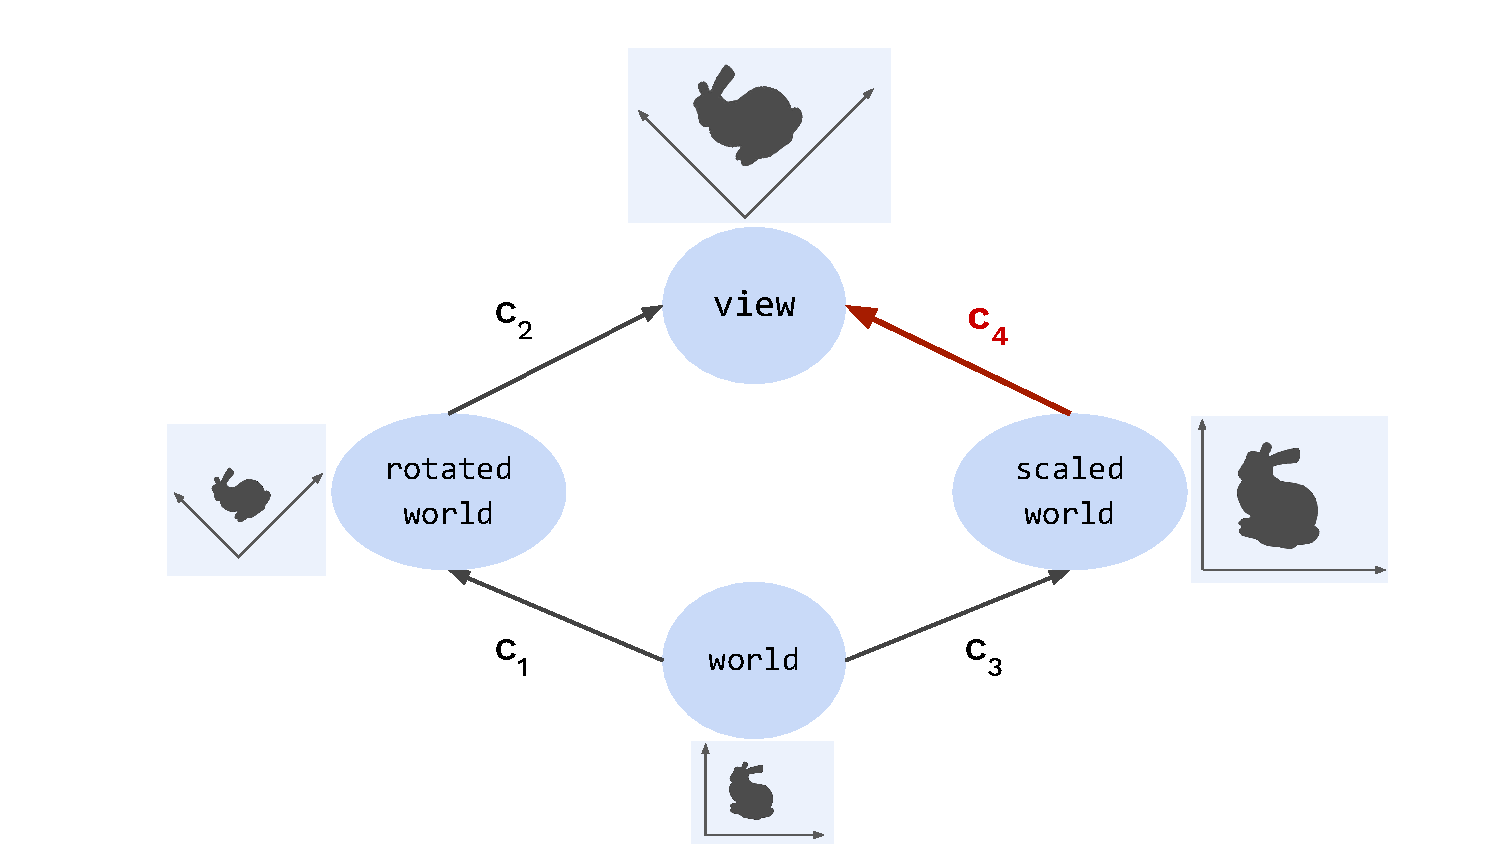
\includegraphics[width=3in]{fig/canonical.pdf}
		\caption{A \emph{transformation graph} with provided transformations. The highlighted edge represents a newly added transformation function, which must be unique and agree with the existing paths on the graph.}
		\label{fig:inpaths}
	\end{minipage}
	\begin{minipage}{.48\linewidth}
		\begin{align*}
			c &\in\text{constants}\\
			x &\in\text{variables}\\
			f &\in \text{function names}\\
			p &\in\text{primitives}\\
			t &\in\text{types} \\
			\tau &\defas \textrm{unit} \,|\, \top_p \,|\, \bot_p \,|\, t \\
			e &\defas v \,|\, c \,|\, f(e_1, e_2) \,|\, x\ \textrm{as!}\ \tau \,|\, x\ \textrm{in}\ \tau\\
			C &\defas \tau \, x = e \,|\, e\\
			P  &=  C;P \,|\, \epsilon\\
		\end{align*}
		\caption{Core Gator syntax.}
		\label{fig:syntax}
	\end{minipage}
\end{figure}
\paragraph{Implementation}
The Gator compiler implements \code{in} expressions by searching for transformations to complete the chain from one type to another.
It uses a \emph{transformation graph} where the vertices are types and the edges are transformation matrices or functions.
Figure~\ref{fig:inpaths} gives a visual representation of a transformation graph.

\subsection{Canonical Functions}
\label{sec:canon}

The transformations that gator reasons about for automatic application are special: they must uniquely define a map from their domain to their range. 
Gator requires these functions to be labeled with the word \code{canon}.
Gator defines three requirements on these transformations:
(1) there can be only one canonical function between each pair of types in a given scope, (2) all canonical functions between reference frames must map between frames of the same dimension, and (3) a canonical function can only have one non-canonical argument.

To expand on condition (3); canonical functions may take in \emph{canonical arguments}, which are variables labelled with the \code{canon} keyword.  The most familiar example of this use is defining matrix---vector multiplication to be canonical; the matrix itself must be included and must be a canonical matrix:
%
\begin{verbatim}
	with frame(3) target:
	canon point *(canon transformation<target> t, point x) {
		...
	}
	...
	// Now declare the matrix as canonical 
	// for use with multiplication
	canon hom<model>.transformation<world> uModel;
	homPos in world; // --> uModel * homPos
\end{verbatim}
%
It is legal to manually fill canonical arguments to functions with non-canonical variables; however, \code{in} expressions will never do so.

The intuition of canonical functions comes from affine transformations between frames and coordinate schemes.
Since each frame has underlying basis vectors, transformations between frames of the same dimension which preserve these frames are necessarily unique; further, applying these bijective transformations does not cause data to ``lose information.''
Similarly, coordinate schemes simply provide different ways to view the same information; there are often unique transformations between schemes that can be applied as needed to unify data representation.

This construction of canonical functions and automatic transformations is similar to constructions provided by C\# and C++'s type coercion.
The slightly different approach needed for \code{in} expressions will be discussed briefly in Section~\ref{sec:rw}.

\subsection{Correctness of Generated Transformations}

With \code{in} expressions, Gator programmers sacrifice control for convenience:
the compiler picks which transformation functions and matrices to use to get from one coordinate system to another.
%
If all the individual transformations marked with \code{canon} are correct, then the composed ``chain'' generated for an \code{in} expression must also be correct.
%
Functional verification of transformations, however, is not feasible in Gator's purely static setting:
it would require not only the value of every transformation matrix, which typically varies dynamically over time,
but also an intrinsic description of each coordinate system, such as the basis vectors for every reference frame, which is never available in real graphics code.
%
We view heavyweight dynamic debugging aids for checking transformation correctness as important future work.

We can, however, state a simple consistency condition that is necessary but not sufficient for a system of canonical transformations to be correct.
%
The transformation system should be \emph{path independent:}
for any two types $\tau_1$ and $\tau_2$, the behavior of any chain of transformations from $\tau_1$ to $\tau_2$ should be equivalent.
%
In other words, every edge in the transformation graph corresponds to a function---so every path corresponds to a function composition,
and every such path between the same two vertices should yield the same composed function.
%
(This definition is equivalent to commutativity for diagrams~\cite{murota}.)
%
Otherwise, the semantics of an expression \code{$e$ in $\tau$} would depend on the graph search algorithm that Gator uses to find routes in the transformation graph, which is clearly undesirable.

Because it is a purely static system, Gator does not enforce path independence.
%
However, path independence motivates Gator's requirement that canonical transformations preserve dimensionality (see Section~\ref{sec:canon}).
%
Without this condition, we have found it is easy to accidentally violate path independence with non-invertible functions and result in an ambiguous transformation graph for \code{in} expressions.
\section{Formal Semantics}
\label{sec:semantics}

% The name of the GLSL-like "target" language.
\newcommand{\targlang}{Hatchling\xspace}

Gator provides a framework for defining geometry types as an ``overlay'' on top of computation-oriented programs in a base language without geometry types.
In this section, we formalize a core of Gator to show that its constructs are sound with respect to such an underlying language.
The goal is a theorem stating that well-typed Gator programs, when translated, result in well-typed programs in the target language.
We focus on the generic, extensible Gator language rather than formalizing the rules for any specific geometric system---affine transformations on Cartesian coordinates, for example.
Proving soundness with respect to a linear algebra domain would be interesting future work but is out of scope for this paper.

We define two languages: a high-level core semantics for Gator that includes its user-defined types, and a low-level abstract target language, \targlang.  \targlang represents a sound imperative language with some set of primitive types and operators on those types.
For example, an instance with fixed-size vector and matrix types can reflect a simple core of GLSL.

\subsection{Syntax}

Figure~\ref{fig:syntax} lists the syntax of the formal core of Gator that we formalize in this section.
The types in this core language consist of \code{unit} and a lattice over each primitive type $p$.
The choice of primitives is kept abstract in this formalism to highlight that the Gator extend over arbitrary underlying datatypes.
For example, in a GLSL core language, we might have a primitive \code{float} or \code{vec3} -- something like \code{vector} would be a custom type $t$ and not a primitive.

A program in Gator is a series of commands; we simplify these to variable declaration, assignment, and expressions.
Gator expressions are constructed around function applications, with \code{as} and \code{in} expressions to help manage types..
We assume functions always take two arguments for simplicity; extending this assumption for other argument counts is straightforward.


\subsection{Typing Rules}
\label{subsec:order}

We define a typing judgment for Gator programs, $\Gamma |- P : \tau$, that, for any program $P$ and typing context $\Gamma$, produces a type $\tau$.  The complete semantics for this judgment can be seen in Figure~\ref{fig:typing}.  
Note that $\Gamma$ is kept constant throughout; declaring a variable requires looking up into the constant $\Gamma$ to determine if the declared type matches the expected type.
Keeping $\Gamma$ constant will later help with translation; the type of any expression can be determined exactly from the constant global contexts $\Gamma,\mathrm{X},\text{and }\Phi$ along with the judgment \textrm{P}.

Gator requires a lattice for each primitive type; custom types on each lattice introduces new subtyping relations.
We define a type ordering among types $\leq$ where $t_1 \leq t_2$ means that $t_1$ is a subtype of $t_2$.
$\leq$ is expected to be reflexive and transitive.
In a well formed program, $\leq$ must contain a rule for every user defined type, every type (except unit) must be a subtype of a primitive top type, and every bottom type $\bot_p$ must be a subtype of each subtype of the associated $\top_p$.
In other words, $\leq$ must conform to a lattice structure for each primitive $p$.
The complete summary of subtyping rules can be found in the attached supplementary materials.

\begin{figure}
	\begin{mathpar}
		\inferrule
		{\tau_1\leq\tau_2\qquad\Gamma\vdash e:\tau_1}
		{\Gamma\vdash e:\tau_2}
		
		\inferrule
		{\textrm{X}(c)=p}
		{\Gamma\vdash c:\bot_p}
		
		\inferrule
		{\Gamma(v)=\tau}
		{\Gamma\vdash x :\tau}
		
		\inferrule
		{\Gamma\vdash e : \tau\qquad\Gamma(v)=\tau}
		{\Gamma\vdash \tau\ x = e:\textrm{unit}}
		
		\inferrule
		{\Gamma\vdash C : \tau_1\qquad\Gamma\vdash P : \tau_2}
		{\Gamma\vdash C;P:\textrm{unit}}
		
		\inferrule
		{ }
		{\Gamma\vdash \epsilon:\textrm{unit}}
		
		\inferrule
		{\Gamma\vdash e: \top_p\qquad\tau\leq\top_p}
		{\Gamma\vdash e\ \textrm{as!}\ \tau:\tau}
		
		\inferrule
		{\Gamma\vdash e : \tau_1\qquad\textrm{P}(\tau_1,\tau_2)=f}
		{\Gamma\vdash e\ \textrm{in}\ \tau_2:\tau_2}
		
		\inferrule
		{\Gamma\vdash e_1:\tau_1\qquad\Gamma,\vdash e_2:\tau_2 \qquad \Phi(f,\tau_1,\tau_2)=\tau_3}
		{\Gamma\vdash f(e_1,e_2):\tau_3}
	\end{mathpar}
	\caption{Typing Judgment}
	\label{fig:typing}
\end{figure}

The typing information for functions is stored in a function typing context, $\Phi$, which maps the tuple of function name and input types to the output type.  The semantics of $\Phi$ are built to support overloaded functions.

Gator, as defined in these semantics, is parameterized over primitive types stored in primitive type context $X$, which maps a literal to its primitive type.

The map from $\mathrm{in}$ expressions to paths is managed by the judgment $\mathrm{P}$.  More precisely, $\mathrm{P}$ maps a given start and end type $\tau_1$ and $\tau_2$ to a function name that, when applied to an expression of type $\tau_1$, produces an expression of type $\tau_2$.  We simplify the judgment of \textrm{P} here to only allow one step for notation clarity; in the real Gator implementation, the transformation may be a chain of functions.  The details of this judgment $\mathrm{P}$ are omitted for simplicity, but amount to a simple lookup through the available functions for a function of the correct type.

\subsection{Translation Soundness}
\begin{figure}
	\begin{align*}
		\source{c}_\Gamma &\triangleq c &
		\source{x}_\Gamma &\triangleq x \\
		\source{\tau\ x := e}_\Gamma &\triangleq \source{\tau}\ x := \source{e}_\Gamma &
		\source{e\ \mathrm{as!}\ \tau}_\Gamma&\triangleq \source{e}_\Gamma \\
		\source{e\ \mathrm{in}\ \tau_2}_\Gamma&\triangleq \source{f(e)}_\Gamma&\text{where }&\Gamma|-e:\tau_1\text{ and }f=\mathrm{P}(e,\tau_1,\tau_2)\\
		\source{f(e_1, e_2)}_\Gamma&\triangleq f'(e_1, e_2)&\text{where }&\Gamma|-e:\tau_1,\Gamma|-e:\tau_2,\text{ and }f'=\Psi(f,e_1,e_2,\tau_1,\tau_2)\\
		\source{\epsilon}_\Gamma&\triangleq \epsilon&
		\source{C;P}_\Gamma&\triangleq\source{C}_\Gamma;\source{P}_\Gamma\\
		\source{t}&\triangleq \top_p&\text{where }t&\leq\top_p\\
		\source{\top_p}&\triangleq \top_p &
		\source{\bot_p}&\triangleq \top_p \\
		\source{\textrm{unit}}&\triangleq \textrm{unit}
	\end{align*}
	\caption{Translational semantics for expressions and types}
	\label{fig:translation}
\end{figure}

To prove the translation soundness of Gator, we need to first define \targlang and our translation from Gator to \targlang.
We will show that a well-typed Gator program must translate to a well-typed \targlang program. 

Primitives in Gator can be translated to a type in the target language. 
For notation convenience we name primitives such that $\top_p$ in Gator translates to $\top_p$ in \targlang.

We define the syntax of \targlang to be identical to Gator syntax except for $\tau$, which is instead written as $\tau::=\mathsf{unit}\,|\,\top_p$, and without $\textrm{as!}$ or $\textrm{in}$ expressions.
In other words, \targlang is simply Gator with custom type labels and associated operations erased.
In the formalism of \targlang, abstraction over operation implementation is done using operation context $\Xi$ that maps an operator name to its output type.

When \targlang is parameterized to be a simple core of GLSL, some top types we might see are the \code{float} and \code{vec3} types.  Translation from Gator would consist of erasing custom geometry types, such as \code{cart3<model>.point}, to their associated top type; in this case \code{vec3}.

To translate Gator's externally-defined functions (which may be overloaded on types not part of \targlang), we invoke the context $\Psi$. 
$\Psi$ maps the tuple of a function name, input expressions, and input types to an expression in the target language. 
For example, we might map Gator's definition of subtraction between points to be a GLSL subtraction between two \code{vec3}s.
The resulting function names must each be unique and preserve the translation of Gator's primitive types.
A well formed function translation context $\Psi$ would necessarily map functions to expressions of the correct return type, as constrained by $\Phi$ under translation.

We reuse the judgment $\mathrm{P}$ as a mechanism to resolve $\mathrm{in}$ expressions, applying the function result of evaluating the judgment to $e$.  This must produce a result of the correct translated type for a well-formed judgment \textrm{P}.

The typing rule for operation expressions is:
%
\begin{mathpar}
	\infer[]
	{\Gamma\vdash o(e_1,e_2):\tau_3}
	{\Gamma\vdash e_1:\tau_1\qquad\Gamma,\vdash e_2:\tau_2 \qquad\Xi(o)=\tau_3}
\end{mathpar}
%
We emphasize this rule as being similar to Gator's rules for operations, but with a ``translated'' context using only \targlang (i.e. primitive) types.  We also note that $\Xi$ does not take in types as arguments, thus \targlang does not support overloaded functions.

We define translational semantics from type-annotated Gator to \targlang in Figure~\ref{fig:translation}. 
The typing contexts $\Gamma$ and $\Phi$ are translated by replacing every $\tau$ in their range with $\llbracket\tau\rrbracket$.

Using structural induction over expressions in Gator, we are now able to show that
\begin{theorem}[translational soundness]
	For all $\Gamma$, $e$, and $\tau$,
	if $\Gamma |- e : \tau$
	then $\source{\Gamma} |- \source{e}_\Gamma : \source{\tau}$.
\end{theorem}
That is to say, if Gator code type checks, then \targlang code type checks.  
Since \targlang is constrained to be sound, Gator must be sound.
A sketch of this proof is included in the provided supplementary materials.
% %
% Appendix~\ref{app:formalism} gives the full translation and proves dimensional safety.

\section{Implementation}
\label{sec:practice}

We implemented Gator in a compiler that statically checks user-defined geometric type systems as described in Section~\ref{sec:langlang} and automatically generates transformation code as described in Section~\ref{sec:in}.
The compiler consists of 2,800 lines of OCaml.
It can emit either GLSL or TypeScript source code, to target either GPU shaders or CPU-side setup code, respectively.

The rest of this section describes how the full Gator language implementation extends the core language features to enable real-world graphics programming.
We demonstrate these features in detail in a series of case studies in Section~\ref{sec:inpractice}.

\subsection{Practical Features}
\label{sec:target}
\paragraph{Types}

While Gator is designed around geometry types, writing realistic code requires a more complete language design.
Aside from the primitive types \code{bool}, \code{int}, \code{float}, and \code{string}, Gator supports fixed-length array types, such as \code{float[3]}, and type aliases.

New types may be declared as a \emph{subtype} of an existing type.
For instance, we can add support for the GLSL-style \code{vec3}:
%
\begin{lstlisting}
type vec3 is float[3];
\end{lstlisting}
%
Through creating a custom type alias, we can, for example, provide support for a subtype of \code{float[3]}, the GLSL \code{vec3}.
While the built-in \code{float[3]} type does not support vector addition, we will be able to write $x+y$ for \code{vec3}s $x,y$ as in GLSL.

To allow literal values to interact intuitively with custom types, literals in Gator have special types.
For example, the number $42$ is of type \code{%int}.
Gator introduces a typing rule where each literal type $\%p$ is a subtype of every subtype of $p$.  In other words, the literal type $\%p$ is the bottom type for the type hierarchy with top type $p$.
We summarize these ideas in this example:
%
\begin{lstlisting}
type vec3 is float[3];
vec3 s1 = [4.2, 4.2, 4.2];  // Legal 
float[3] x = s1;            // Legal
vec3 s2 = x;                // ERROR: float[3] is not a vec3
\end{lstlisting}
%
This behavior of literal values allows us to capture the Gator-style intuition that a given vector can either be a geometric point or just a raw GLSL \code{vec3}, but this information is not known until the data is assigned to a variable.
\paragraph{Type Inference}
Gator supports local type inference using the \code{auto} keyword:
%
\begin{lstlisting}
cart3<model>.point fragPos = ...;
// worldPos will have type cart3<world>.point
auto worldPos = fragPos in world;
\end{lstlisting}
%
\paragraph{External Functions}
Functions and variables defined externally in the Gator target can be written using the \code{declare} keyword.
%
\begin{lstlisting}
declare vec3 normalize(vec3 v);
\end{lstlisting}
%
All arithmetic operations in Gator are functions which can be declared and overloaded.
Gator has no built-in functions.
Requiring this declaration allows us to include GLSL-style infix addition of vectors without violating coordinate systems restrictions:
%
\begin{lstlisting}
	declare vec3 +(vec3 v1, vec3 v2);
\end{lstlisting}
%
Addition is then valid for values of type \code{vec3}:
%
\begin{lstlisting}
vec3 x = [0., 1., 2.];
vec3 result = x + x; // Legal
\end{lstlisting}
%
But emits an error when applied to two points, as desired, since they are not subtypes of vec3 and so there is no valid function overload:
%
\begin{lstlisting}
cartesian<model>.point fragPos = [0., 1., 2.];
// ERROR: No addition defined for points
auto result = fragPos + fragPos; 
\end{lstlisting}
%
\paragraph{Import System}
To support using custom Gator libraries in a readable way, we built a simple import system in Gator.  Files can be imported with the keyword \code{using} followed by the name of the file:
%
\begin{lstlisting}
using "../glsl_defs.lgl";
\end{lstlisting}
%
\paragraph{Unsafe Casting}
As an escape hatch from strict vector typing, Gator provides an unsound cast expression written with \code{as!}:
%
\begin{lstlisting}
vec3 position = fragPos as! vec3;
\end{lstlisting}
%
Casts must preserve the primitive representation; we could not, for instance, cast a variable with type \code{float[2]} to \code{float[3]}.
Unsafe casts syntactically resemble \code{in} expressions but are unsound and carry no run-time cost.
These casts both allow for unsafe transformations for defining a function that is externally ``known'' to be safe, and for allowing the user to forgo Gator's type system and work directly with GLSL-like semantics, as seen in the example above.

\subsection{Standard Library}
Per Section \ref{sec:semantics}, Gator does not include any built-in functions or operations.  Our implementation does provide array indexing as a built-in function to help simplify definitions, but otherwise matches requires that operations such as \code{+} be explicitly declared.

We implement a standard library provides access to common GLSL operations.  This library consists of GLSL function declarations, scheme declarations for Cartesian and Homogeneous coordinates, and basic transformation functions such as \code{homify} and \code{reduce}.  Relevant GLSL functions are declared to work on GLSL types, such as the addition operation operation in section~\ref{sec:practice}:
%
\begin{lstlisting}
declare vec3 +(vec3 x, vec3 y);
\end{lstlisting}
%
We build schemes in much the same way as introduced in Section~\ref{subsec:schemes}, as with the sketch of the \code{cart3} scheme:
%
\begin{lstlisting}
with frame(3) r:
coordinate cart3 : geometry {
  object vector is float[3];
  vector +(vector v1, vector v2) {
	return [
	  v1[0] + v2[0], 
	  v1[1] + v2[1], 
	  v1[2] + v2[2]];
  }
}
\end{lstlisting}
%
Finally, we include \code{homify} and \code{reduce} transform between homogeneous and cartesian coordinates as discussed in Section~\ref{subsec:objects}:
%
\begin{lstlisting}
hom<model>.point homify(cart3<model>.point p) {
  return [p[0], p[1], p[2], 1.]; 
}
cart3<model>.point reduce(hom<model>.point p) {
  return [p[0], p[1], p[2]]; 
}
\end{lstlisting}
%
We use this same library when implementing each shader for the case study.
\section{Gator in Practice}
\label{sec:inpractice}

This section explores how Gator can help programmers avoid geometry bugs using a series of case studies.
We use the Gator compiler to implement OpenGL-based renderers that demonstrate a variety of common visual effects,
and we compare against implementations in plain GLSL.
We report qualitatively on how Gator's type system influences the expression of the rendering code (Section~\ref{sec:casestudies} and quantitatively on the performance impact of Gator's \code{in} expressions (Section~\ref{sec:performance}).

\subsection{Case Studies}
\label{sec:casestudies}

\begin{figure}
\centering
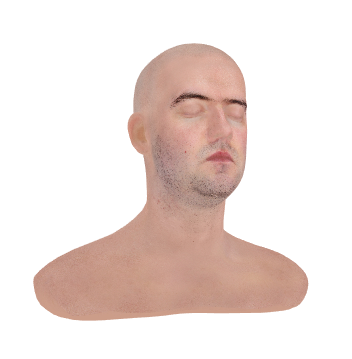
\includegraphics[width=\linewidth]{fig/texture.png}
\caption{Texture.}
\label{fig:texture}
\end{figure}
\begin{figure}
		\centering
		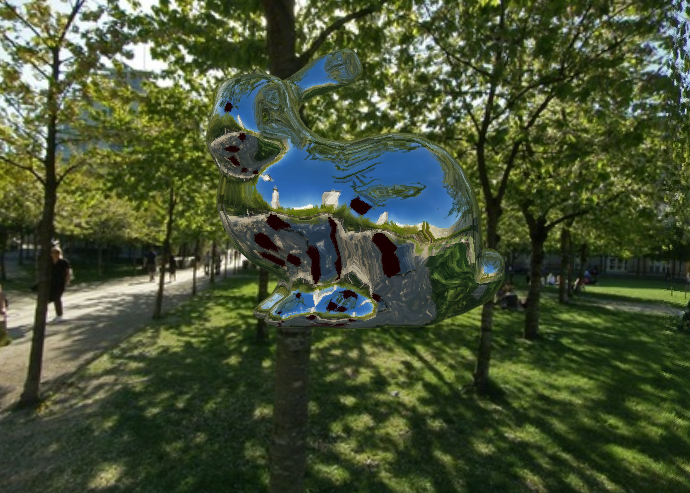
\includegraphics[width=\linewidth]{fig/reflection.png}
		\caption{Reflection.}
		\label{fig:reflection}
\end{figure}
	
\begin{figure}
		\centering
		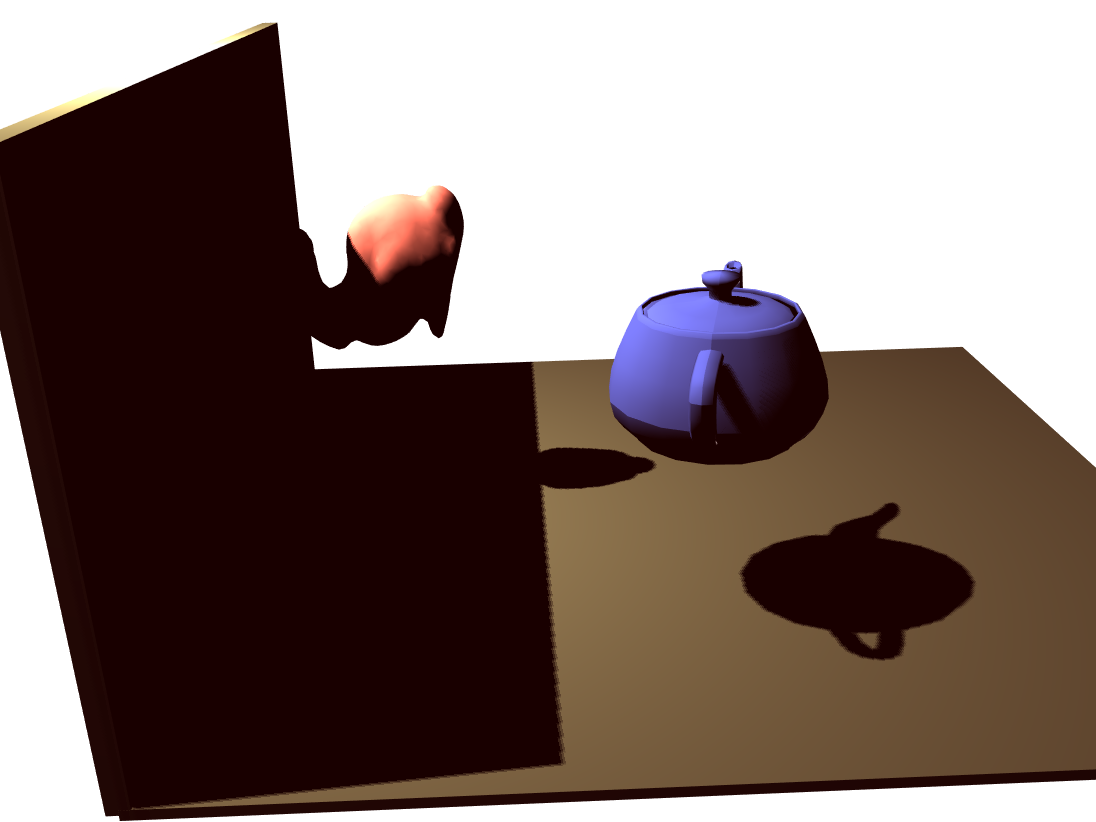
\includegraphics[width=\linewidth]{fig/shadowmap.png}
		\caption{Shadow map.}
		\label{fig:shadowmap}
\end{figure}
\begin{figure}
		\centering
		
\includegraphics[width=\linewidth]{fig/microfacet.png}
		\caption{Microfacet.}
		\label{fig:microfacet}
\end{figure}

% This stuff seems like a rehash of things we've already said above---no need
% to repeat. --A
% To evaluate Gator's expressiveness and effectiveness at ruling out geometry bugs, we implemented a compiler from Gator to GLSL and used it to create a series of standard shader implementations.
% To help normalize the differences between Gator and GLSL, we include a GLSL-specialized standard library and basic import system as described above in section~\ref{sec:target}.

To qualitatively study Gator's safety and expressiveness, we used it to implement 8 renderers based on the OpenGL API in its browser-based incarnation, WebGL~\cite{webgl}.
To the best of our knowledge, there is no standard benchmark suite for evaluating the expressiveness and performance of graphics shader programs.
Instead, we assemble implementations of a range of common rendering effects:
%
\begin{itemize}
	\item \emph{Phong:} The lighting model introduced in Section~\ref{sec:example}.
	\item \emph{Reflection:} Use two-pass rendering to render an object that reflects its surroundings.
	\item \emph{Shadow map:} Simulate shadows for moving objects by computing a projection.
	\item \emph{Microfacet:} Texture model for simulating roughness on a surface.
	\item \emph{Texture:} Use OpenGL's texture mapping facility to draw an image on the surface of an object.
	\item \emph{Spotlight:} Phong lighting restricted to a spotlight circle.
	\item \emph{Fog:} Lighting model with integration to simulate distortion from fog.
	\item \emph{Bump map:} Texture model for simulating bumps on surfaces.
	%\item \emph{Multiple lights:} Multiple lights with shadows to stress geometry transformations.
\end{itemize}
%
Each renderer consists of both CPU-side ``host'' code and several GPU-side shader programs.
Figure~\ref{fig:examples} depicts the output of a selection of these renderers.
% I wrote this sentence but I think it's superfluous. --A
% We compare against baseline implementations using TypeScript and GLSL to show how Gator's type system can eliminate potential pitfalls in those standard languages.

The rest of this section reports on salient findings from the case studies and compares them to standard implementations in GLSL and TypeScript.
For the sake of space, we highlight the most distinct cases where Gator helped clarify geometric properties and prevent geometry bugs that would not be caught by plain GLSL.  The complete code of both the Gator and reference GLSL implementations can be found online.\footnote{URL omitted for anonymous review}

\paragraph{Reflection}

Our reflection case study, shown in Figure~\ref{fig:reflection}, renders an object that reflects the dynamic scene around it, creating a ``mirrored'' appearance.
The surrounding scene includes a static background texture, known as a \emph{skybox}, and several non-reflective floating objects to demonstrate how the reflected scene changes dynamically.

Rendering a reflection effect requires several passes through the graphics pipeline.
The idea is to first render the scene that the mirror-like object will reflect, and then render the scene again with that resulting image ``painted'' onto the surface of the object.
There are three main phases:
(1) Render the non-reflective objects from the perspective of the reflective object.
This requires six passes, one for each direction in 3-space.
(2) Render the reflection using the generated cube as a texture reference.
(3) Finally, render all other objects from the perspective of the camera.

\paragraph{Reflection: Inverse Transformation}
For the second step, we refer to a cubemap---a special GLSL texture with six sides---to refer to the six directions of the scene.  
To calculate the angle of reflection, we need to reason about the interactions of the light rays in view space \emph{as they map onto our model space}.  
Specifically, calculating the reflection amounts to the following operations, where \code{V} is the current vertex's position and \code{N} is the current normal vector, which must both be in the view frame:
%
\begin{lstlisting}
uniform samplerCube<alphaColor> uSkybox;
...
void main() {
  ...
  cart3<view>.vector R = -reflect(V, N);
  auto gl_FragColor = textureCube(uSkybox, R in model);
}
\end{lstlisting}
%
The key feature to note here is the transformation \code{R in model}, which accomplishes our goal of returning the light calculation to the object's perspective (the model frame).
This transformation requires that we map backwards through the world frame, a transformation which requires the inverse of the \code{model}$\rightarrow$\code{world} matrix and the \code{world}$\rightarrow$\code{view} matrix multiplied together.
This interaction produces a unique feature in Gator's type system, where we need to both have a forward transformation and its inverse.
The shader declares the matrices as follows, with the inversion being done preemptively on the CPU:
%
\begin{lstlisting}
canon uniform hom<world>.
  transformation<view> uView;
canon uniform hom<model>.
  transformation<world> uModel;
canon uniform cart3<view>.
  transformation<model> uInverseViewTransform;
\end{lstlisting}
%
The inverse view transform uses a Cartesian (\code{cart3}) matrix because
we intend only to use it for the vector \code{R}, which ignores the translation component of the affine transformation.  The inverse transformation is what permits us to write \code{R in model}, while the forward transformations must be uniquely given to actually send our position and normal to the view frame (as noted before):
%
\begin{lstlisting}
varying cart3<model>.point vPosition;
varying cart3<model>.normal vNormal;
void main()
auto N = normalize(vNormal in view);
auto V = -(vPosition in view);
...
}
\end{lstlisting}
%
\paragraph{Reflection: Normal Transformation}
Additionally, we need to reason about the correct transformation of the normal \emph{with translation} (that is, when moving the object in space), which means that we need the inverse transpose matrix, which provides a distinct path between the model and view frames.  The use of the inverse transpose of the model-view matrix is perhaps unexpected; it arises specifically for a geometry normal from a convenient algebraic result.

In GLSL, it is easy to mistakenly transform the normal as if it were an ordinary direction:
%
\begin{lstlisting}
varying vec3 vNormal;
void main() {
  auto N = normalize(vec3(
    uView * uModel * vec4(vNormal, 0.)));
}
\end{lstlisting}
%
This code is wrong because \code{uModel * vec4(vNormal, 0.)} does not apply the translation component of the \code{uModel} transformation.
To prevent this kind of bug, the Gator standard library defines the \code{normal} type, which is a subtype of \code{vector}.
A new \code{normalTransformation} type can only operate on normals.
Using these types, a simple \code{in} transformation suffices:
%
\begin{lstlisting}
canon uniform cart3<model>.
  normalTransformation<view> uNormalMatrix;
varying cart3<model>.normal vNormal;
void main() {
  // uNormalMatrix * vNormal
  auto N = normalize(vNormal in view);  
}
\end{lstlisting}
%
The compiler uses the normal version of the transformation, correctly applying the translation component.

\paragraph{Shadow Map: Light Space}
Shadow mapping is a technique to simulate the shadows cast by 3D objects when illuminated by a point light source.  Our case study, shown in Figure~\ref{fig:shadowmap}, renders several objects that cast shadows on each other and a single ``floor'' surface.  The non-shadow coloring is simulated through Phong lighting as previously discussed.

As with the reflection renderer, to calculate shadows in a scene, we require several passes through the graphics pipeline.  The first pass renders the scene from the perspective of the \emph{light} and calculates the whether a given pixel is obscured by another.  The second pass uses this information to draw shadows; a given pixel is lit only if it is not obscured from the light.

The first pass does all geometric operations in the vertex shader to render the scene from the light's perspective.  This is easy to get wrong in GLSL by defaulting to the usual transformation chain:
%
\begin{lstlisting}
void main() {
  // The usual transformation chain here is wrong!
  // We should instead be using 
  //    uLightProjective and uLightView
  vec4 gl_Position = uProjective * 
    uView * uModel * vec4(aPosition, 1.);
}
\end{lstlisting}
%
This incorrect transformation chain will lead to shadows in strange places and hard-to-debug effects.

In Gator, on the other hand, the work is done when typing the matrices themselves.  From there, the transformation to light space is both documented and correct by construction:
%
\begin{lstlisting}
attribute cart3<model>.point aPosition;
canon uniform hom<model>.
  transformation<world> uModel;
canon uniform hom<world>.
  transformation<light> uLightView;
canon uniform hom<light>.
  transformation<lightProjective> uLightProjection;

void main() {
auto gl_Position = aPosition in hom<lightProjective>;
// ...
}
\end{lstlisting}
We use the depth information in the final pass in the form of \code{uTexture}.  To look up where the shadow should be placed, we must lookup the position of the current pixel in the light's projective space (which is where the position was represented in the previous rendering).
In GLSL, we require the following hard-to-read code:
\begin{lstlisting}
float texelSize = 1. / 1024.;
float texelDepth = texture2D(uTexture, 
vec2(uLightProjective * uLightView * 
  uModel * vec4(vPosition, 1.))) + texelSize));
\end{lstlisting}
Using the correct transformations is difficult and hard to be sure if the correct transformation chain was used once again.  In Gator, on the other hand, this is straightforward:
\begin{lstlisting}
float texelSize = 1. / 1024.;
float texelDepth = texture2D(uTexture, 
  vec2(vPosition in lightProjective) + texelSize));
\end{lstlisting}

\paragraph{Microfacet: Custom Canonical Functions}

Anisotropic microfacet shading creates an illusion of roughness and bumpiness on a 3D modeled surface using information from the normal map of that surface.  Modeling this correctly, however, requires an unusual technique: building a local reference frame from the perspective of the normal vector called the local normal frame.

Converting to the local normal frame of a given normal consists of a function call with the appropriate normal vector.
%
\begin{lstlisting}
vec3 proj_normalframe(vec3 m, vec3 n) { ... }
vec3 geom_normal;
vec3 result = proj_normalframe(viewDir, geom_normal);
\end{lstlisting}
%
However, as with other conversions between spaces,
writing this kind of code in GLSL can
involve multiple nonobvious steps.
If the normal and target direction are in different spaces, the GLSL code must look like this:
%
\begin{lstlisting}
vec3 result = proj_normalframe(vec3(uView * 
  uModel * vec4(modelDir, 1.)), geom_normal);
\end{lstlisting}
%
In Gator, we instead declare \code{proj_normalframe} with the appropriate types and a canonical tag, noting that the normal itself is a canonical part of the transformation:
%
\begin{lstlisting}
frame normalframe has dimension 3;
canon cart3<normalframe>.direction proj_normalframe(
cart3<view>.direction m, canon cart3<view>.normal n) { ... }
\end{lstlisting}
%
We then declare the normal \code{geom_normal} with the appropriate type, and the transformation type becomes straightforward:
%
\begin{lstlisting}
canon cart3<view>.normal geom_normal;
auto result = modelDir in normalframe;
\end{lstlisting}
%
\paragraph{Textures: Parameterized Types}
A \emph{texture} is an image that a renderer maps onto the surface of a 3D object, creating the illusion that the object has a ``textured'' surface.
Our texture case study renders a face mesh with a single texture (shown in Figure~\ref{fig:texture}).
While this example does not provide any geometry insight, we highlight the study to show the broad utility of the types introduced by Gator for a graphics context.
GLSL represents a texture using a \code{sampler2D} value, which acts as a pointer to the requested image, which is typically an input to a shader:
%
\begin{lstlisting}
uniform sampler2D uTexture;
\end{lstlisting}
%
Textures are mapped to the image using the object's current texture coordinate:
%
\begin{lstlisting}
varying vec2 vTexCoord;
\end{lstlisting}
%
Whereas textures themselves are typically constant (using the \code{uniform} keyword), a texture coordinate like \code{vTexCoord} differs for each vertex in a mesh (as the \code{varying} keyword indicates).
To sample a color from a texture at a specific location, a fragment shader must use the GLSL \code{texture2D} function:
%
\begin{lstlisting}
vec4 gl_FragColor = texture2D(uTexture, vTexCoord);
\end{lstlisting}
%
The result type of \code{texture2D} in GLSL is \code{vec4}: while textures typically contain colors (consisting of red, green, blue, and alpha channels), renderers can also use them to store other data such as shadow maps or even points in a coordinate system.

In Gator and its GLSL standard library, \code{sampler2D} is a polymorphic type that indicates the values it contains:
\begin{lstlisting}
with float[4] T:
declare type sampler2D;
with float[4] T:
declare T texture(sampler2D<T> tex, vec2 uv);
\end{lstlisting}
For this renderer, the texture contains \code{alphaColor} values, which represent color values that can be used as \code{gl_FragColor}.
The fragment shader is nearly identical to GLSL but with more specific types:
%
\begin{lstlisting}
uniform sampler2D<alphaColor> uTexture;
varying vec2 vTexCoord;
void main() {
  alphaColor gl_FragColor = texture2D(uTexture, vTexCoord);
}
\end{lstlisting}
%
With this code, we guarantee that the texture represented by \code{uTexture} will produce a color which can be directly used by \code{gl_FragColor}.  We therefore both provide documentation and prevent errors with trying to use the resulting vector as, say, a point for later calculations.

\subsection{Performance}
\label{sec:performance}

While Gator is chiefly an ``overhead-free'' wrapper that expresses the same semantics as an underlying language,
there is one exception where Gator code can differ from plain GLSL:
its automatic transformation insertion using \code{in} expressions (Section~\ref{sec:in}).

The Gator implementation compiles \code{in} expressions to a chain of transformation operations that may be slower than the equivalent in a hand-written GLSL shader.
In particular, hand-written GLSL code can store and reuse transformation results or composed matrices, while the Gator compiler does not currently attempt to do so.
The Gator compiler also generates function wrappers to enable its overloading.
While both patterns should be amenable to cleanup by standard compiler optimizations,
this section measures the performance impact by comparing Gator implementations of renderers from our case study to hand-optimized GLSL implementations.

\subsubsection{Experimental Setup}

We perform experiments on Windows 10 version 1903 with an Intel i7-8700K CPU, NVIDIA GeForce GTX 1070, 16 GB RAM, and Chrome 81.0.4044.138.
We run 60 testing rounds, each of which executes the benchmarks in a randomly shuffled order.
In each round of testing, we execute each program for 20 seconds while recording the time to render each frame.
We report the mean and standard deviation of the frame rate across all rounds.

\subsubsection{Performance Results}

\begin{figure}
\centering
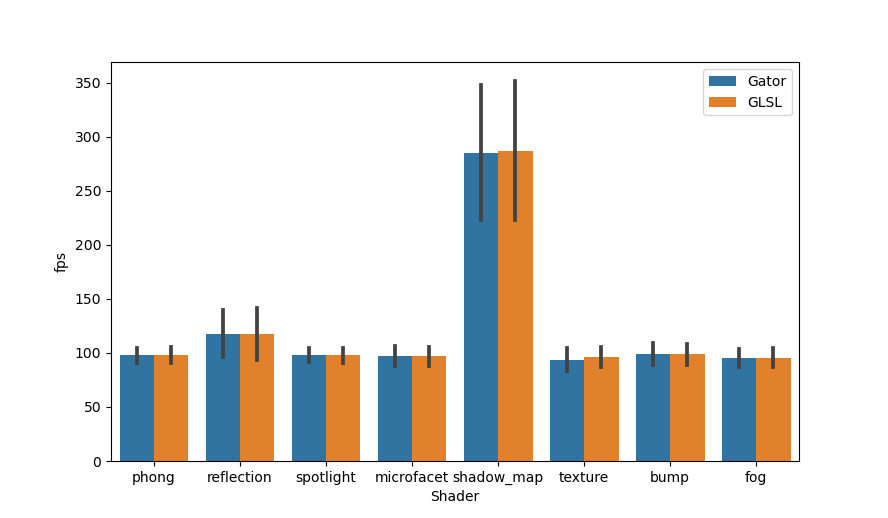
\includegraphics[width=\linewidth]{fig/evalresultsgator.png}
\caption{The mean frames per second (fps) for each shader for both the baseline (GLSL) and Gator code. Error bars show the standard deviation.}
\label{fig:runtime-results}
\end{figure}
\begin{figure}
\centering
\begin{tabular}{ccccccc}
& \multicolumn{2}{c}{Gator} & \multicolumn{2}{c}{GLSL} & \multicolumn{2}{c}{$p$-value} \\
\cmidrule(r){2-3} \cmidrule(r){4-5} \cmidrule(r){6-7}
Shader & Mean & S.E. & Mean & S.E. & Wilcoxon & TOST \\
\midrule
\bmark{phong}      & 97.84 & 0.22 & 97.67 & 0.21 & 0.187    & 0.003*\\
\bmark{texture}    & 95.82 & 0.27 & 93.75 & 0.31 & $<$0.001*& 0.996\\
\bmark{reflect}    & 117.8 & 0.72 & 117.7 & 0.65 & 0.638    & 0.188\\
\bmark{shadow}     & 287.0 & 1.91 & 285.1 & 1.85 & 0.365    & 0.636\\
\bmark{bump}       & 98.60 & 0.29 & 99.07 & 0.29 & 0.063    & 0.098\\
\bmark{microfacet} & 96.71 & 0.27 & 96.91 & 0.28 & 0.640    & 0.020*\\
\bmark{fog}        & 95.74 & 0.26 & 95.41 & 0.25 & 0.119    & 0.033*\\
\bmark{spotlight}  & 97.83 & 0.21 & 98.07 & 0.20 & 0.299    & 0.005*\\
\bottomrule
\end{tabular}
\captionof{table}{Mean and standard error of the frame rate for the Gator and GLSL (baseline) implementation of each benchmark. We also give the $p$-value for a Wilcoxon sign rank test and two one-sided $t$-test (TOST) equivalence test that checks whether the means are within 1~fps, where * denotes statistical significance ($p < 0.05$).}
\label{tab:perf-results}
\end{figure}

Figure~\ref{fig:runtime-results} shows the average frames per second (fps) for the GLSL and Gator versions of each renderer, and Table~\ref{tab:perf-results} shows mean and standard deviation of each frame rate.
The frame rates for the two versions are generally very similar---the means are all within one standard deviation.
% within 1~fps, except for \bmark{shadow}, which has a particularly high variance, and \bmark{texture}, which we discuss in more detail below.
Several benchmarks have frame rates around 100~fps because they render the same number of objects and the bulk of the cost comes from scene setup.
% Many of the results appear clustered around 100~FPS; this is due to testing taking place with similar number of objects for each.
% While the shaders provide variation in frame rate, the bulk of the frame cost is the size of the scene being setup.
We used around 100 objects for all scenes except \bmark{reflection} and \bmark{shadow} to reduce natural variation and focus on measuring the cost of the shaders.

Table~\ref{tab:perf-results} shows the results of Wilcoxon signed-rank statistical tests that detect differences in the mean frame rates.
At an $\alpha = 0.05$ significance level, we find a statistically significant difference only for \bmark{texture}.
However, a difference of means test cannot \emph{confirm} that a difference does \emph{not} exist.
For that, we also use we use the two one-sided $t$-test (TOST) procedure~\cite{tost}, which yields statistical significance ($p < \alpha$) when the difference in means is within a threshold.
We use a threshold of 1~fps.
The test rejects the null hypothesis---concluding, with high confidence, that the means are similar---for the \bmark{phong}, \bmark{microfacet}, \bmark{fog}, and \bmark{spotlight} shaders.

The anomaly is \code{texture}, where our test concludes that a small (2~fps) performance difference does exist, although the differences are still within one standard deviation.
Our best guess as to the reason is due to a result of the boilerplate functions inserted by Gator, some of which be optimized away with more work.

\section{Related Work}
\label{sec:rw}

SafeGI~\cite{safegi} introduces a type system as a C/C++ library for geometric objects parameterized on reference frame labels not unlike Gator's geometry types.  The types introduced by SafeGI do not include information about the coordinate scheme, and so also requrie abstracting the notion of transformations to a map type which must be applied through a layer of abstraction.  
Additionally, SafeGI does not attempt to introduce automatic transformations like Gator's \code{in} expressions nor attempt to study the result of applying these types to real code.

The dominant mainstream graphics shader languages are OpenGL's GLSL~\cite{glsl} and Direct3D's HLSL~\cite{direct3d}.
Research on graphics-oriented languages for manipulating vectors dates at least to Hanrahan and Lawson's original \emph{shading language}~\cite{hanrahan90}.
Recent research on improving these shading languages has focused on modularity and interactions between pipeline stages:
Spark~\cite{spark} encourages modular composition of shaders;
Spire~\cite{spire} facilitates rapid experimentation with implementation choices;
and Braid~\cite{braid} uses multi-stage programming to manage interactions between shaders.
These languages do not address vector-space bugs.
Gator's type system and transformation expressions are orthogonal and could apply to any of these underlying languages.

Scenic~\cite{spatial} introduces semantics to reason about relative object positions and $\lambda$CAD~\cite{acad} introduces a small functional language for writing affine transformations, although neither seem to have a type system for checking the coordinate systems they've defined.
Practitioners have noticed that vector-space bugs are tricky to solve and have proposed using a naming convention to rule them out~\cite{naming}.
A 2017 enumeration of programming problems in graphics~\cite{lfogl} identifies the problem with latent vector spaces and suggests that a novel type system may be a solution.
Gator can be seen as a realization of this proposal.

Gator's type system works as an overlay for a simpler, underlying type system that only enforces dimensional restrictions.
This pattern resembles prior work on type qualifiers~\cite{cqual}, dimension types~\cite{dimension}, and type systems for tracking physical units~\cite{unit}.
Canonical transformations in Gator are similar in feel to Haskell's type class polymorphic functions, where Gator's \code{space} type can be defined as a type class and the \code{in} keyword behave similarly to Haskell lookup calls.
Additionally, Gator's notion of automatic transformations is a specialized use type coercion, similar to structures introduces in the C\# and C++ languages.
What is particular about Gator's automatic type coercion is the notion of path independence discussed in Section~\ref{sec:in}, along with a definition of uniqueness and bijectivity of canonical transformations. Together, these requirements allow automation of coordinate system transformations that would not be allowed in other, similar systems.

\section{Conclusion}

Gator attacks a main impediment to graphics programming that makes it hard to learn and makes rendering software hard to maintain.
Geometry bugs are extremely hard to catch dynamically, so Gator shows how to bake them into a type system and how a compiler can declaratively generate ``correct by construction'' geometric code.
We see Gator as a foundation for future work that brings programming languages insights to graphics software,
such as formalizing the semantics of geometric systems
and providing abstractions over multi-stage GPU pipelines.

Geometry bugs are not just about graphics, however.
Similar bugs arise in fields fields ranging from robotics to scientific computing.
In Gator, users can write libraries to encode domain-specific forms of geometry: affine, hyperbolic, or elliptic geometry, for example.
We hope to expand Gator's standard library as we apply it to an expanding set of domains.

\bibliography{venues,refs}
